\apendice{Especificación de diseño}

\section{Introducción}
En este apartado se documentan los datos , la arquitectura, el procedimiento y la guía de estilo del proyecto.
\section{Diseño de datos}

El almacenamiento de datos se realiza en un fichero CSV denominado \texttt{webhook\_dataset.csv}, generado y mantenido por la aplicación Flask. Cada fila del fichero representa un conjunto de datos recibidos de TTN.

Los campos de los datos recibidos son los siguientes:

\begin{itemize}
    \item \textbf{timestamp}: Fecha y hora de recepcion del mensaje.
    \item \textbf{occupied (boolean)}: Indica si se detectó movimiento en su campo de visión.
    \item \textbf{button\_pressed (boolean)}: Estado del botón del sensor.
    \item \textbf{tamper\_detected (boolean)}: Detección de presencia.
    \item \textbf{battery\_voltage (float)}: Voltaje actual de la batería (V).
    \item \textbf{temperature\_celsius (int)}: Temperatura medida (ºC).
    \item \textbf{humidity\_percent (int)}: Humedad relativa (\%).
    \item \textbf{time\_since\_last\_event\_min (int)}: Minutos desde el último evento.
    \item \textbf{event\_count (int)}: Contador de eventos.
\end{itemize}

Por último, la aplicación añade un campo más (estado) y le otorga el valor correspondiente al resultado obtenido en el análisis del paquete de datos recibido.

Todos los datos son almacenados en texto plano, separados por comas y con codificación UTF-8.

Además, en este proyecto se ha utilizado una base de datos SQL encargada de almacenar y gestionar los credenciales de inicio de sesión de los diferentes usuarios que quieran usar la aplicación.

Por último, cada usuario puede almacenar diversos ficheros csv en su lista de ficheros csv personal. Todo fichero que se encuentre en esa lista podrá ser utilizado por el usuario. para aplicar las diversas funcionalidades de la aplicación. Los ficheros cargados en la aplicación para ser analizados también son guardados en esta lista tras el análisis. 

\section{Diseño arquitectónico}
En este apartado se van a mostrar las distintas estructuras utilizadas durante el desarrollo del proyecto.

\subsection{Modelo-Vista-Controlador (MVC)}

El patrón MVC es un patrón de diseño muy utilizado en aplicaciones web. Divide una aplicación en tres componentes principales:

\begin{itemize}
    \item Modelo: Gestiona los datos (modificar, almacenar\ldots).
    \item Vista: Se encarga de mostrar los datos al usuario. Es la parte visual de la aplicación (interfaz).
    \item Controlador: Intermediario entre la vista y el modelo. Recibe las peticiones del usuario, llama al modelo y selecciona la vista adecuada para la respuesta.
\end{itemize}

\subsubsection{Modelo}
En el proyecto, el Modelo estaría representado por las funciones que leen, procesan y almacenan datos en esos archivos o los propios archivos csv donde se almacenan los datos.

\subsubsection{Vista}
En el proyecto, la Vista estaría representada en las gráficas que la aplicación muestra al usuario tras aplicar un fichero csv o la visualización del contenido de un paquete antes de que el usuario decida enviarlo al dataset.

\subsubsection{Controlador}
En el proyecto, el Controlador estaría representado por los formularios que permiten al usuario introducir valores que serán utilizados por el programa para desempeñar distintas funciones o los botones con los que el usuario puede interactuar para llevar a cabo una acción.

\subsection{Frontend y Backend}

En el proyecto desarrollado se nota una clara diferenciación entre el frontend y el backend. La primera aplicación ,webhook\_flask, está centrada en el backend, mientras que la segunda aplicación ,dashboard\_flask, se centra en el frontend.

\subsubsection{Frontend}
dashboard\_flask es la aplicación encargada de todas las funcionalidades relacionadas con interactuar con el usuario y permitir al mismo disfrutar de la lógica detrás de las funciones del backend sin necesidad de comprender su funcionamiento.

\subsubsection{Backend}
webhook\_flask en cambio es la aplicación más centrada en procesamiento de datos y comprobación de que el flujo de datos con la red LoRaWAN esté funcionando correctamente, para permitir así al usuario disfrutar plenamente de las funciones que ofrece el proyecto.

Esta clara separación entre las dos aplicaciones facilita la organización y mantenimiento del proyecto, además de ayudar al desarrollo de nuevas funcionalidades en el futuro.


\subsection{Arquitectura del proyecto}
La arquitectura final del proyecto desarrollado es:

\imagen{arquitectura}{Arquitectura del proyecto}

Los rectángulos azules hacen referencia a la parte del proyecto más relacionada con una red LoRaWAN, es la parte que no he tenido que desarrollar, sino configurar para asegurar su correcto funcionamiento durante el desarrollo del proyecto.

Los rectángulos amarillos hacen referencia a las dos aplicaciones web que he desarrollado para lograr los objetivos del proyecto.

El rectángulo verde representa el archivo csv denominado webhook\_dataset, el archivo principal del proyecto y con el que ambas aplicaciones interactúan.

Por último, se representa con un rectángulo blanco al usuario, el cual interactúa con el proyecto a través de la primera aplicación web.

\section{Diseño procedimental}
A continuación se muestran distintos diagramas referentes a distintas acciones que se llevan a cabo durante el proyecto.

La \autoref{fig:C2} representa el caso de recepción y almacenamiento de datos.

La \autoref{fig:C3} representa el caso de carga de archivos csv.

\begin{figure}
    \centering
    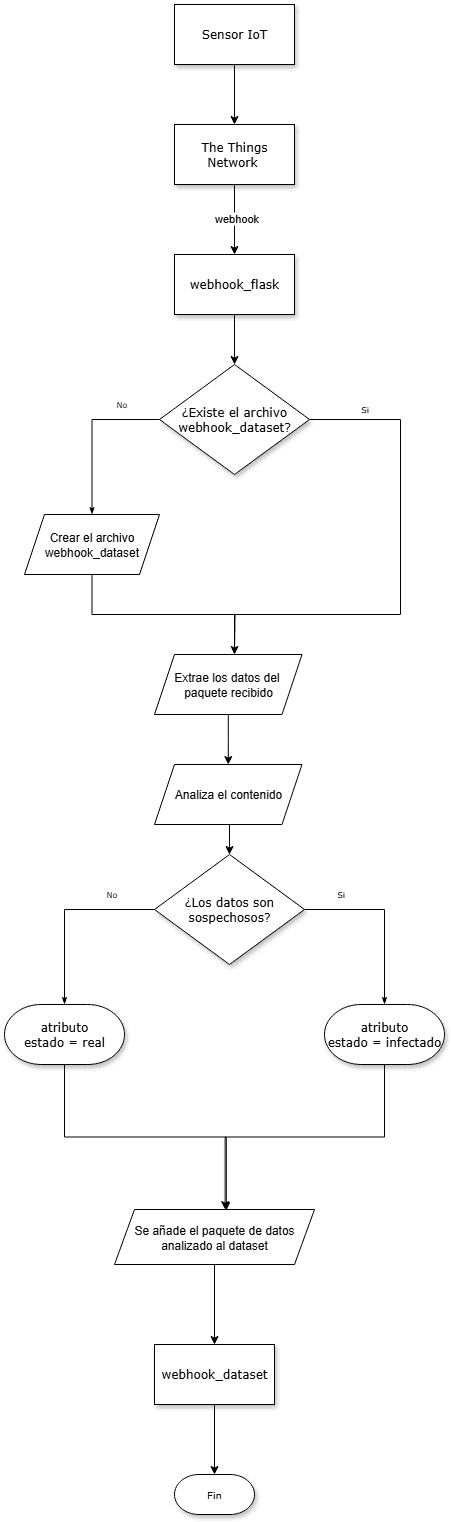
\includegraphics[width=0.5\textwidth]{recibir} 
    \caption{Diagrama de recepción y almacenamiento de datos.}
    \label{fig:C2}
\end{figure}


\begin{figure}
    \centering
    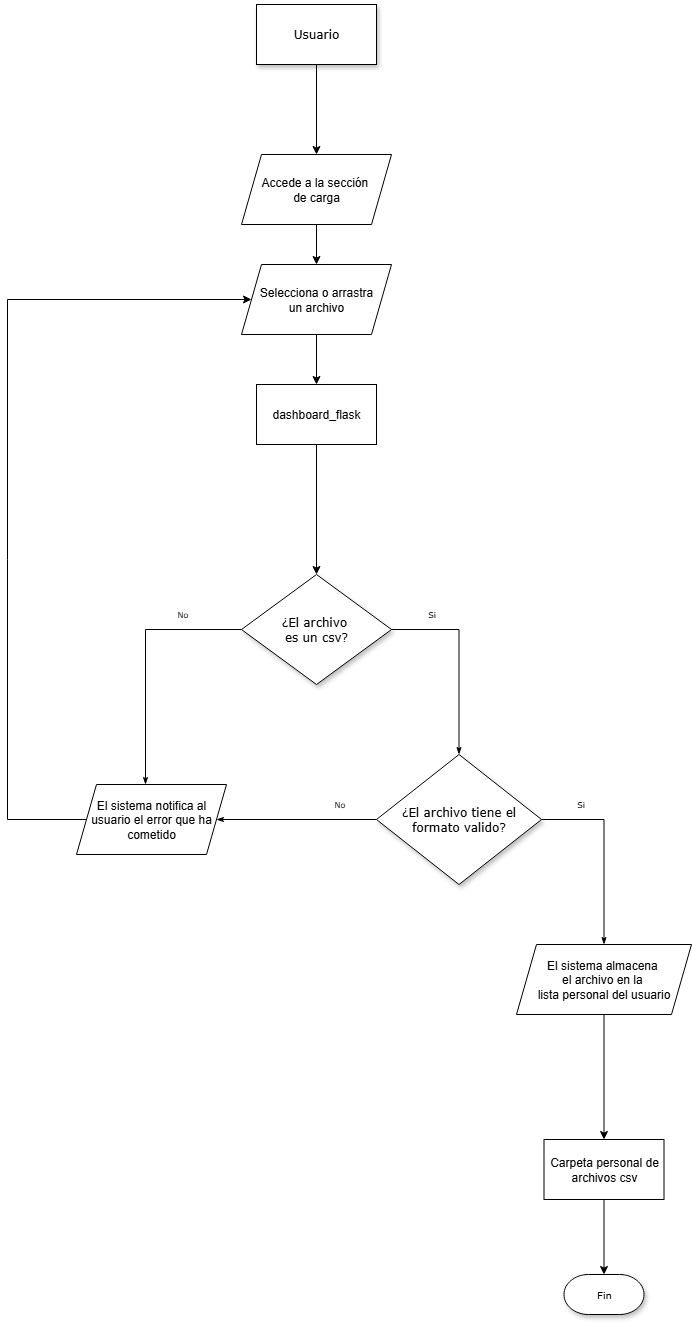
\includegraphics[width=0.8\textwidth]{cargar} 
    \caption{Diagrama de carga de archivos csv.}
    \label{fig:C3}
\end{figure}